\chapter{Construction}

\section{Component List}

\begin{verbatim}
    C1                      68pf
    C2,C3,C6                0.01uf
    C4,C8                   82pf    
    C5                      150pf 
    C7                      22nf    
    C9,C20-26,C28-38,
        C40-45              0.1uf        
    C10                     0.001uf
    C27                     ??
    C39                     47uf 16V

    D1-D5                   1N914 
    
    Q1-Q3                   2N3906 pnp 
    Q4-Q6                   2N3904 npn 
    
    R1,R14,R16,R74,R76      1K
    R2,R4,R10,R12,R26,
        R52,R54,R55,R57,
        R58,R60,R61,R63,
        R65                 10K     
    R3                      100K 
    R5-R9,R15,R18-R25,R62,
        R64,R66             4K7 
    R11,R13,R75             10K POT 
    R17                     5K POT 
    R27                     100
    R28-R45,R53,
        R56,R59,R67         470R 
    R46,R48,R50,R69,
        R71,R73             220R 
    R47,R49,R51,R68,R70,
        R72                 390R    (see note below)

    R77-R84                 ???
    
    U1                      7476 
    U2                      CA3130 
    U3                      6850 
    U4                      6502 
    U5-U9                   2716/28C16 
    U10,U19                 8T26
    U11                     74LS123
    U12,U17,U20,U28,U31     74LS04  (see 2716 mods below)
    U13                     NE555 
    U14                     74LS148 
    U15  (Empty Socket)
    U16                     74LS139 
    U18                     74LS30 
    U21  (Empty Socket)
    U22                     74123
    U23                     7474 
    U24,U25,U32,U41         74LS17 
    U26                     74LS138 
    U27                     74LS10 
    U29                     74LS20 
    U30                     74LS14 
    U33-U40                 2114 
\end{verbatim}

The following Components are not needed if the RS232 is not required, see (\emph{Adding the RS232 Interface}).

\begin{verbatim}
    D3-D5
    Q1-Q6
    R46-R66
    U20
    U30
\end{verbatim}

The 502 CPU has an internal clock oscillator but often derives its clock externally such as from the 540 video card via the bus. This is selected by link W1. The following components are not needed if an external, clock is to be used.

\begin{verbatim}
    C4
    C8
    R10-13
    U11
\end{verbatim}    

\section{Modifications}

\subsection{Board Modifications}

The modifications described here required are required to get the board to function correctly.

\begin{itemize}
\item Cut trace from U22-6 to R75 center pin and install a jumper from R75 center pin to C9.
\item Install Jumper between the two square holes near R26.
\item Fix missing trace on U16 pin 14. It connects to neighbouring trace on top of PCB.
\end{itemize}

\subsection{Using 2716 EPROMS}

The modifications described here are to allow the board to support 2716 EPROMS or 28C16 EEPROMS.

\begin{itemize}
\item Cut trace between U6-18 and U6-21 (component side).
\item Connect U6-18 to U5-18 on (solder side).
\item Above U7, cut bridge at W4 topside and connect center of W4 to other position (ground).
\item Above U9: cut bridge at W8a (there should be no link on W8a, see below).
\item Above U9, connect U9-18 to U8-18 (solder side).
\item Below U8, W5 would normally be moved from its default position to the alternative position. However, if U17 is removed as described below, this is not strictly necessary.
\item U17 (74LS04) is no longer required and can be be removed and replaced by linking pin 3--4, pin 5--6, pin 8--9, pin 10--11 and pin 12--13.
\end{itemize}

W8 is in fact two links, W8a and W8b. Whilst viewing the board with the 48 way bus connector on the right, W8a is the link on the left with W8b being the one on the right.

It is worth noting that some EPROMS have been found not to work in the 502 board. For example, whilst many \emph{\textbf{SGS M2716 F1}} devices seem to work fine, that is not always the case for the \emph{\textbf{SGS M271 F1 Fast}} devices.

\subsection{Adding the RS232 Interface}

The 502 card supports either a cassette interface or a serial interface. In addition, the serial interface can be configured to be TTL levels or RS232 levels.

Fitting resistors R46-R51 and R68-R73 provide a TTL serial I/O at J3 in addition to the cassette interface at J2.

The cassette and the serial interfaces share the same ACIA and in theory can be used simultaneously. However, in practice this can be problematic. When configuring the system for serial use it may be prudent to isolate the cassette interface. This can most easliy be done by removing U23 and U1.

To make the serial interface compatible with an RS232 serial device, the following components need to be fitted.

\begin{verbatim}
    D3-D5
    Q1-Q6
    R46-R66
    U20
    U30
\end{verbatim}

Note the orientation of the transistors as the through holes on the circuit board are positioned the opposite way round for transistors typically supplied in the TO92 package.

In addition R46-R51 and R68-R73 should not be present and the links adjacent to U30 and U41 should be cut. See \textbf{Fig. \ref{fig:u30_links}} and \textbf{Fig. \ref{fig:u41_links}} for details.

\begin{figure}[htbp]
    \begin{center}
    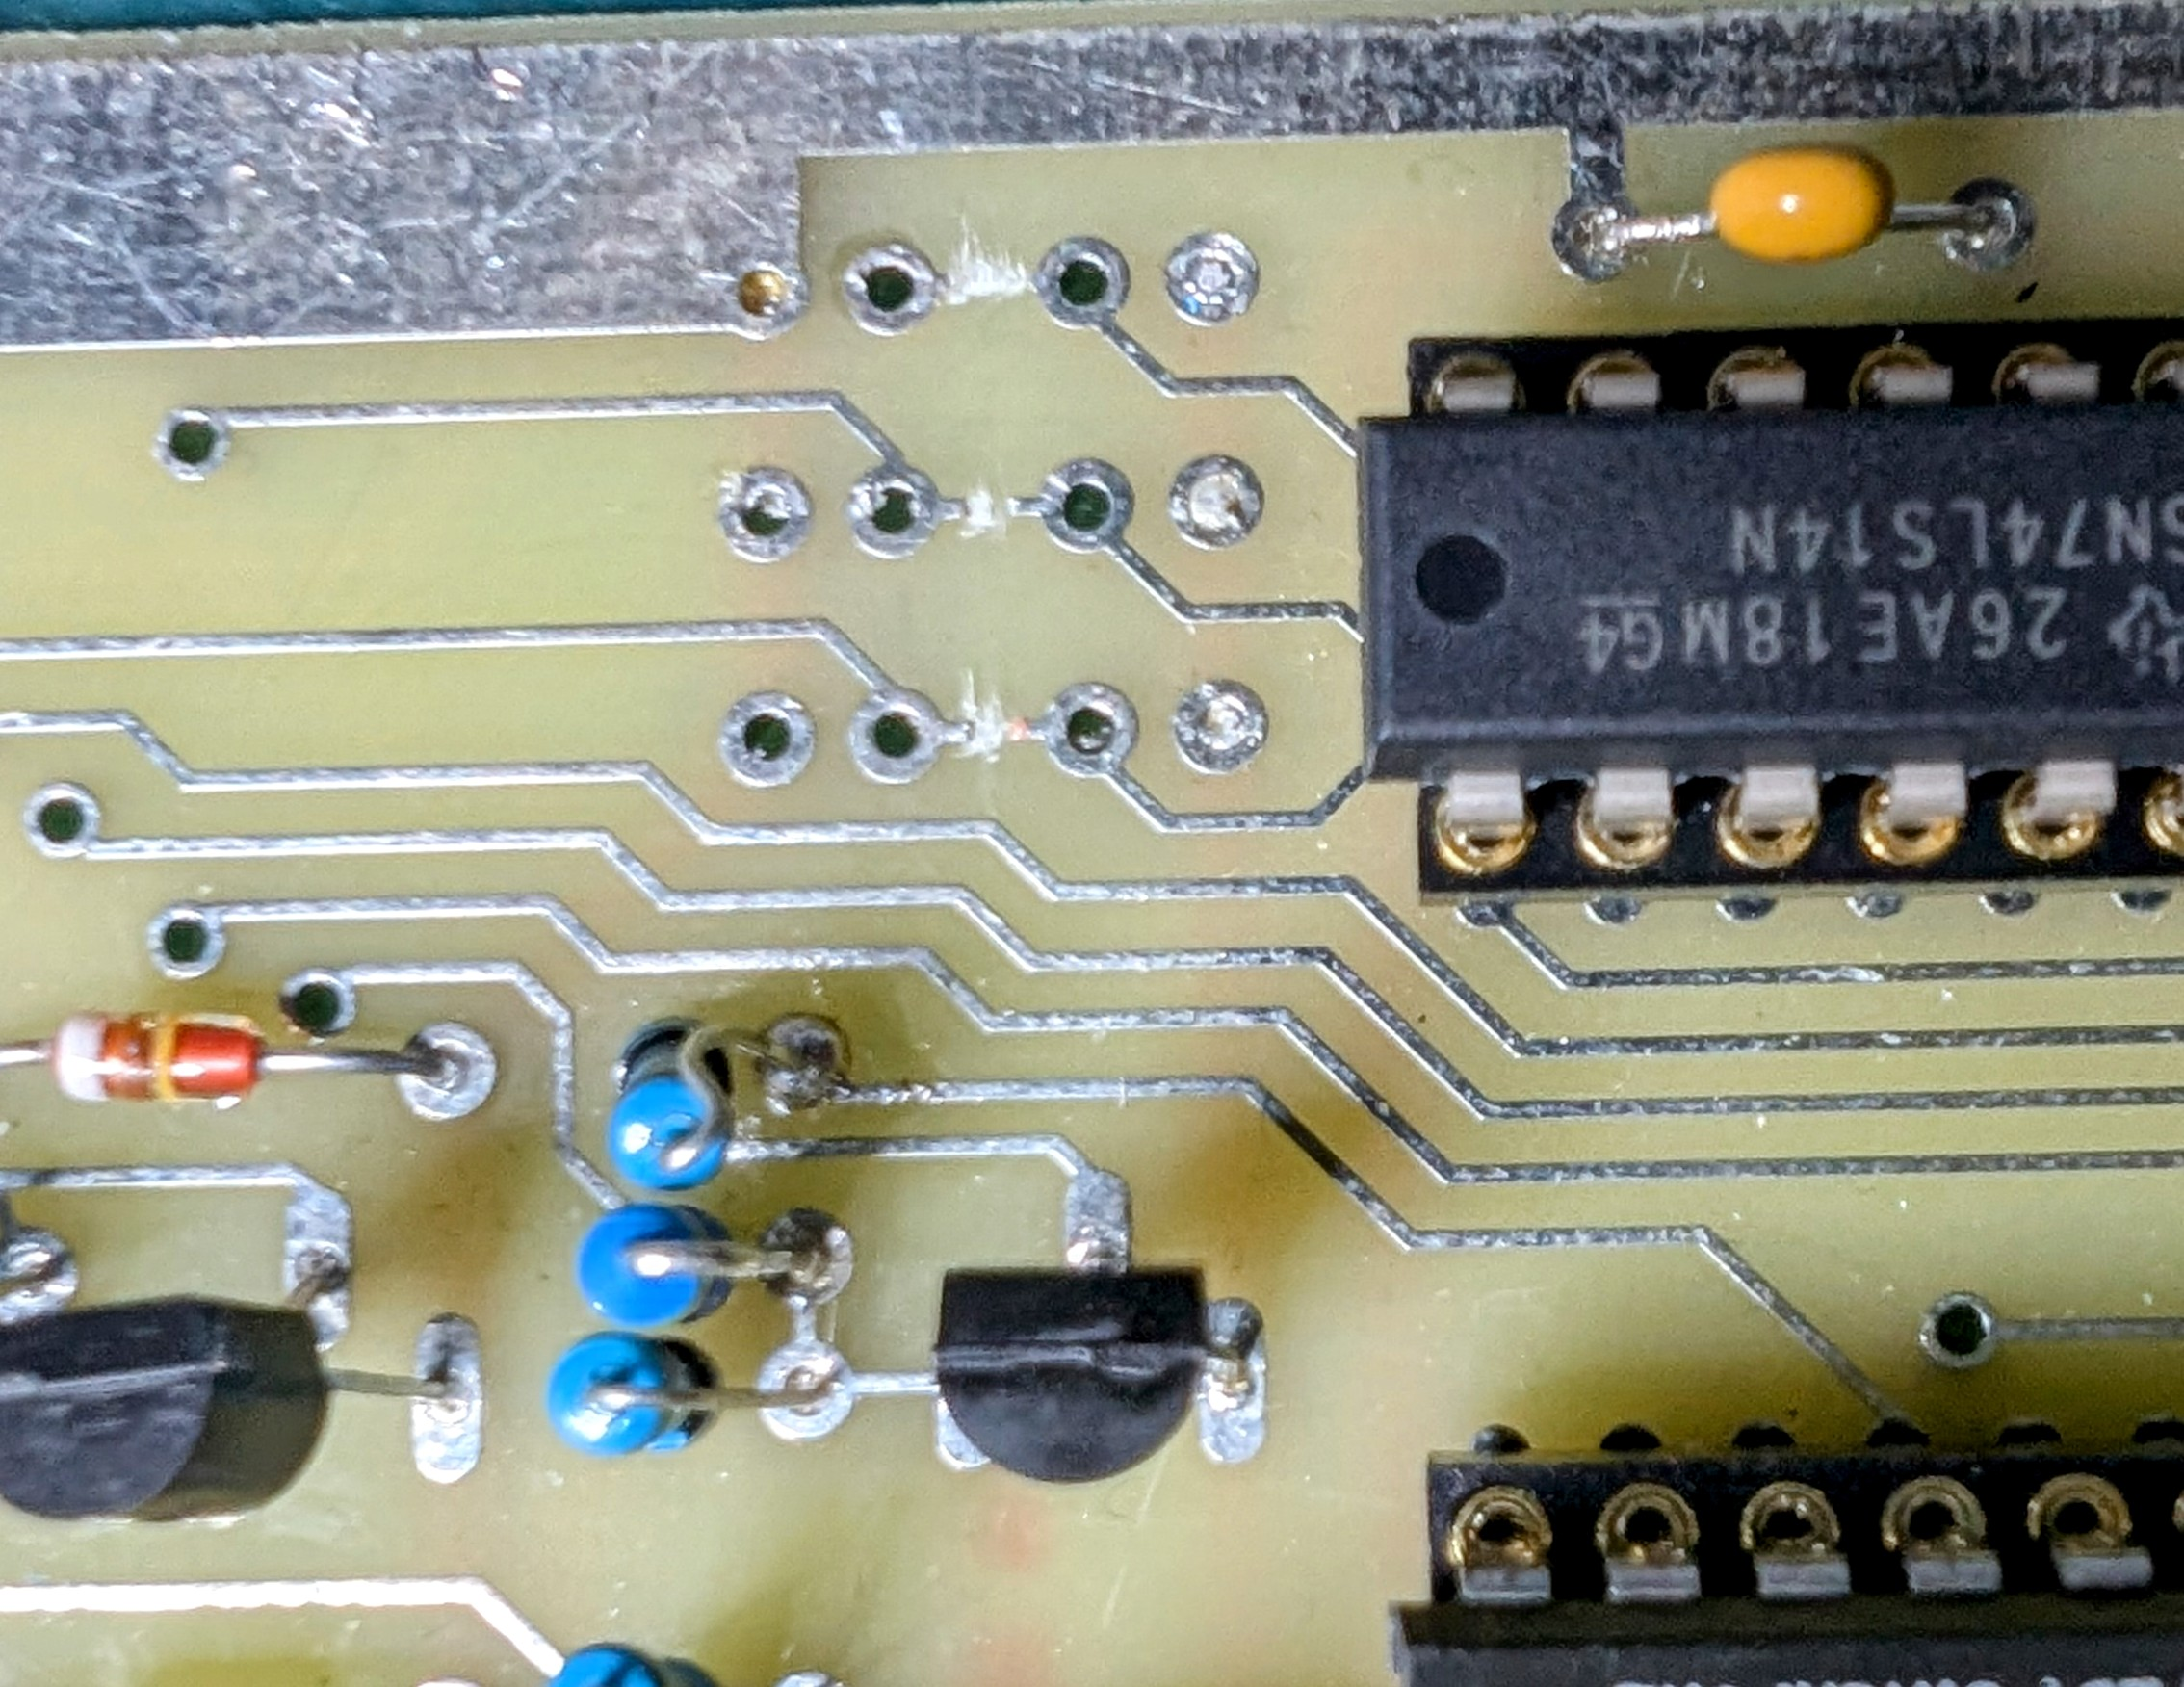
\includegraphics[width=4.9in]{images/U30_links.jpg}
    \caption{Links to be cut just next to U30 on component side.}
    \label{fig:u30_links}
    \end{center}
    \end{figure}

\begin{figure}[htbp]
    \begin{center}
    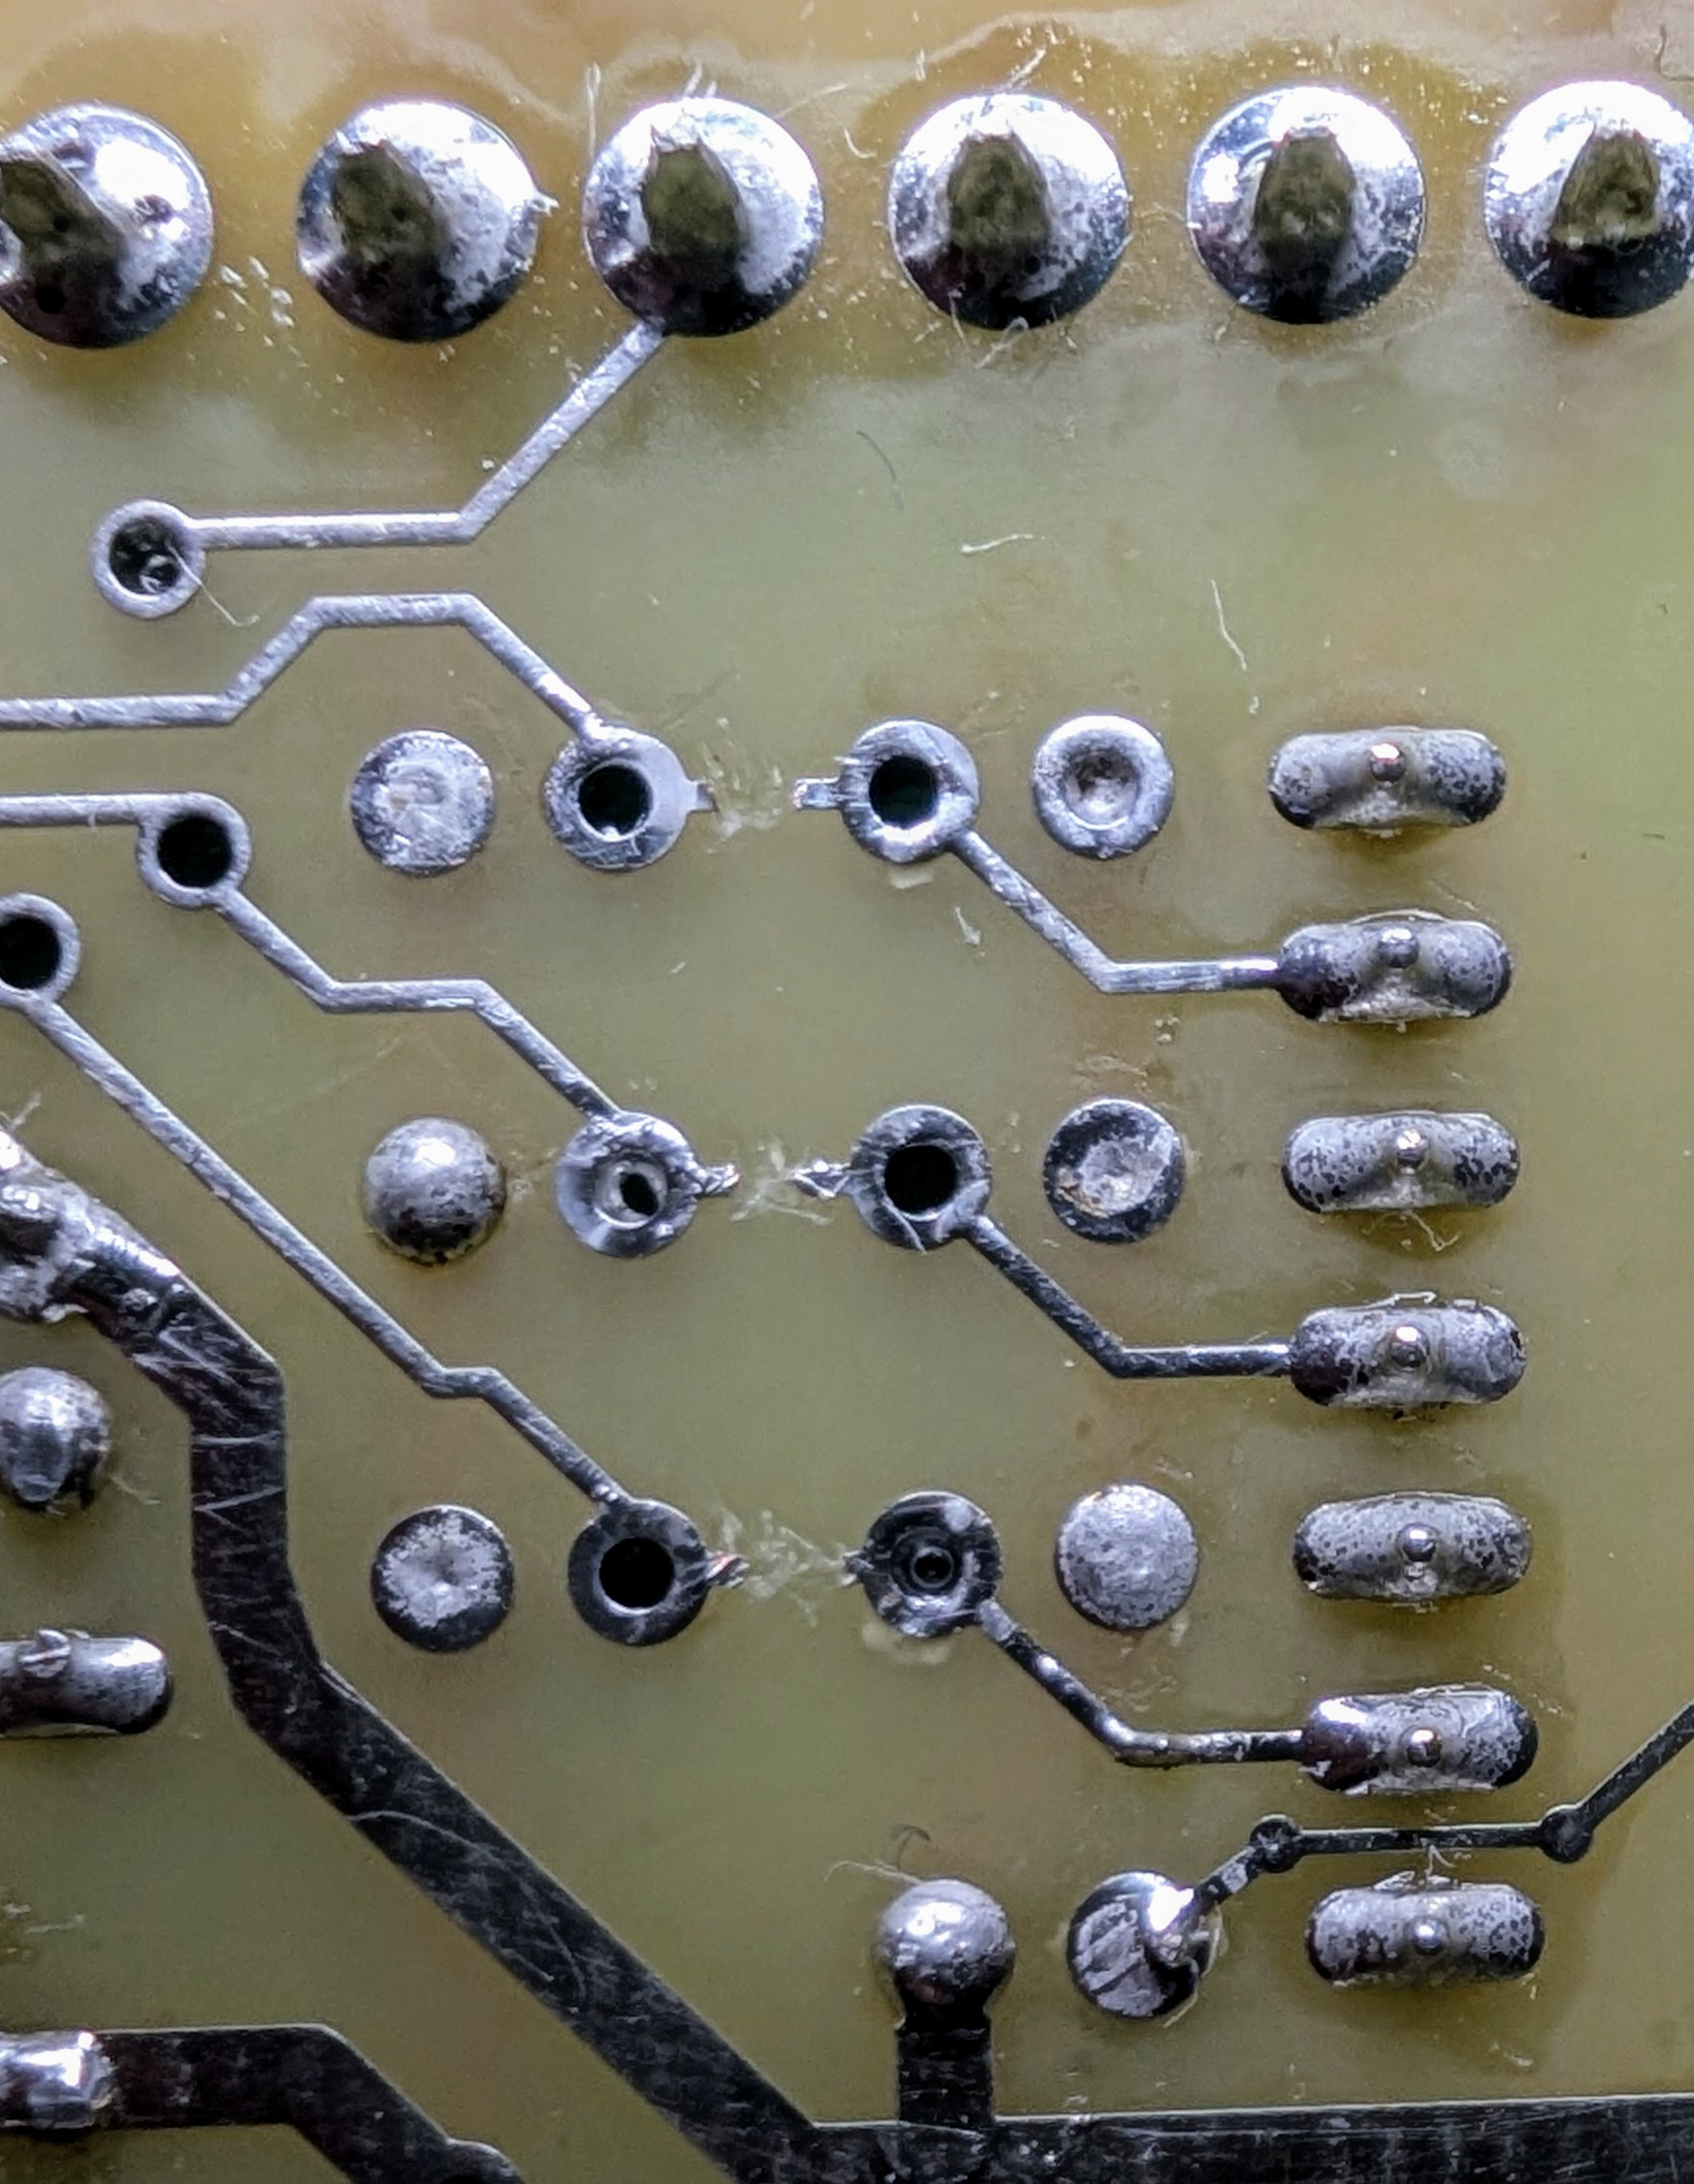
\includegraphics[width=4.9in]{images/U41_links.jpg}
    \caption{Links to be cut just next to U41 on solder side.}
    \label{fig:u41_links}
    \end{center}
    \end{figure}

When configuring the system for RS232 compatibilty it would be prudent to isolate the cassette interface. This can most easliy be done by removing U23 and U1.

The serial interface typically runs at 300 baud with 8 data bits, no parity and 2 stop bits.

Link W3 (see schematic) connects an input presented to J3 pin 7, to be connected to either CTS or DCD on the ACIA if required. With the link in the default position, DCD and CTS inputs to the ACIA are held active (low). 

Link W2 connects the transmit clock output to the receive clock input providing a simple method of setting the receive clock to match the transmit clock. The default position of the link makes this connection.

\section{Monitor Mapping}

\subsection{Overview}

The OSI Monitor ROMs often contain monitor programs for a multitude of machine configurations. Socket U15 on the 502 board allows specific parts of the monitor ROM to be selected as required.

For example a 502 serial system might use the 65A monitor code loaded at FE00 i.e. page 6 of the ROM, and the 65AB Basic Boot code at FF00 i.e page 7 of the ROM. Alternatively a system without ROM basic might simply use the 65A monitor located at FF00 (page 7). Each of these options can be configured using the links at U15.

\subsection{Decoding}

The upper address pages (FDxx, FExx, FCxx) are decoded into separate signals, which are then directed to a 8 line priority encoder (U14). The output of U14 provides the three addresses lines to the ROM. The signals are jumpered to map a particular memory page to a particular ROM page address using the U15 link area.

\begin{figure}[htbp]
    \begin{center}
    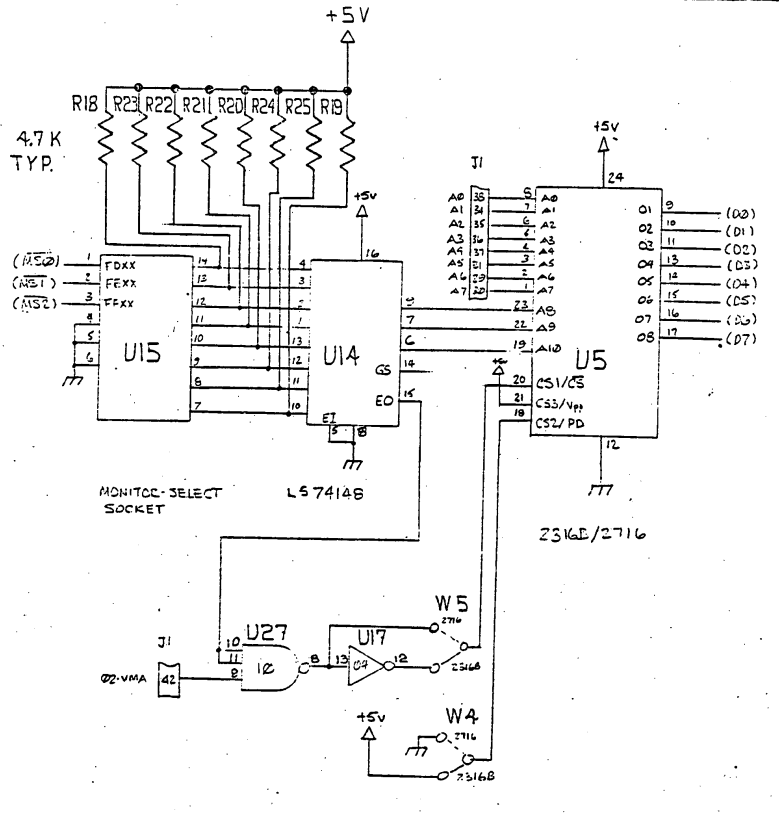
\includegraphics[width=4.9in]{images/Decoder.png}
    \caption{OSI 502 Priority Decoder.}
    \label{fig:decoder}
    \end{center}
    \end{figure}

The output of U14 is inverted, meaning that an input to U14 of '00000000' produces an output of '111'. The outputs are fed as address lines to the monitor ROM. See \textbf{Fig. \ref{fig:decoder}} for details.

Therefore, to map FE00 to page 6 of the ROM and FF00 to page 7 of the ROM, jumpers would be placed on U15 pin 3 to pin 7 and U15 pin 2 to pin 8 (see below).

\subsection*{U15 Pinout}

\begin{verbatim}    
    1 = FDxx selected
    2 = FExx selected
    3 = FFxx selected
    4 = Gnd
    5 = Gnd
    6 = Gnd
    7 = ROM select page 7
    8 = ROM select page 6
    9 = ROM select page 5
    10 = ROM select page 4
    11 = ROM select page 3
    12 = ROM select page 2
    13 = ROM select page 1
    14 = ROM select page 0
\end{verbatim}

\subsection{SYNMON page layout}

\begin{verbatim}
    Page 0 FE00 OSI 440 board 65V monitor (ASCII KB).
    Page 1 FF00 OSI 440 board C/W/M BASIC boot (ASCII KB).
    Page 2 *FD00 C2/540 Polled Keyboard routine.
    Page 3 *FE00 C2/540 65V Monitor.
    Page 4 *FF00 C2/540 BASIC Boot (C/W/M?).
    Page 5 FD00 initializes HDisk controller (CD74/CD36 winchester HD).
    Page 6 FE00/FF00 OSI 65A Serial Monitor.
    Page 7 *FF00 C2/540 disk boot (H/D/M?) works with serial or video.
\end{verbatim}

\subsection{SYN600 - page layout}

\begin{verbatim}
    page 000 'H/D/M' maps to $FF00 for a C2/C4 540Vid disk system.
    page 100 keypoller maps to $FD00 for a C2/C4 540Vid system.
    page 200 monitor maps to $FE00 for a C2/C4 540Vid system.
    page 300 'C/W/M' maps to $FF00 for a C2/C4 540Vid tape system.
    page 400 disk boot maps to $FC00 for a C1 system.
    page 500 keypoller maps to $FD00 for a C1 system.
    page 600 monitor maps to $FE00 for a C1 system.
    page 700 'D/C/W/M' maps to $FF00 for a C1 system.
\end{verbatim}

\subsection{65A-65AB Serial System - page layout}

This card, with the standard addressing scheme would have access to three pages only.

\begin{verbatim}
    Page 5 Free
    Page 6 FE00/FF00 OSI 65A Serial Monitor.
    Page 7 FF00 Basic boot (C/W/M?).
\end{verbatim}

Based on the above, a typical U15 link arrangement for the 502 board would be.

\begin{verbatim}
    Pin 3 to Pin 7  (FF00)
    Pin 2 to Pin 8  (FE00)
    Pin 1 to Pin 9  (FD00)
\end{verbatim}
